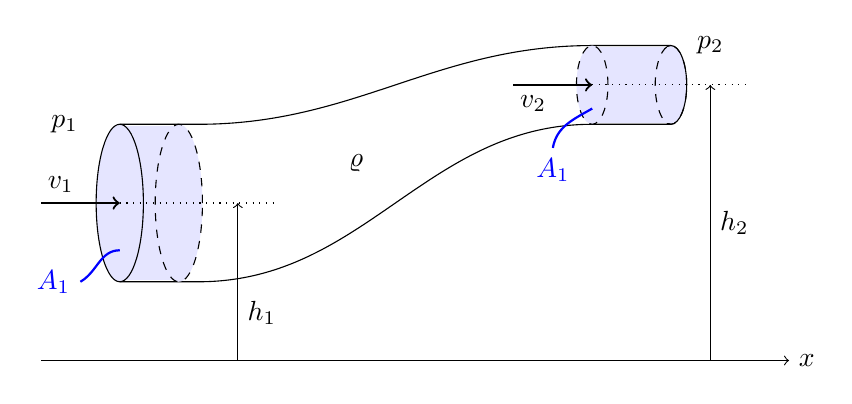
\begin{tikzpicture}
    % axis
    % \draw[->] (-1.5,-1.5) to ++(0,5) node[anchor=south] {\(y\)};
    \draw[->] (-1,-1) to (8.5,-1) node[anchor=west] {\(x\)};
    
    % tube lines
    \draw[] (0,2) to (1,2) to[out=0, in=180] (6,3) to (7,3);
    \draw[] (0,0) to (1,0) to[out=0, in=180] (6,2) to (7,2);
    
    % opening ellipse for A1
    \draw[blue!10, fill=blue!10] (0,.025) rectangle ++(.75,1.95);
    \draw[fill=blue!10] (0,1) ellipse (.3 and 1);
    % ellipse
    \draw[dashed, fill=blue!10] (.75,1) ellipse (.3 and 1);
    % closing ellipse
    \draw[fill=blue!10] (7,2.5) ellipse (.2 and .5);
    %% hide half of the ellipse and make dashed
    \draw[blue!10, fill=blue!10] (6,2.025) rectangle ++(1,.95); 
    \draw[dashed] (7,2.5) ellipse (.2 and .5);
    % ellipse for A2
    \draw[dashed, fill=blue!10] (6,2.5) ellipse (.2 and .5);
    
    % vectors
    \draw[thick, ->] (-1,1) to node[near start, above, anchor=south] {\(v_1\)} ++(1,0) ;
    \draw[thick, ->] (5,2.5) to node[near start, below, anchor=north] {\(v_2\)} ++(1,0) ;
    
    % heights
    \draw[dotted] (0,1) to (2,1);
    \draw[->] (1.5,-1) to node[pos=.3, anchor=west, right] {\(h_1\)} (1.5,1);
    
    \draw[dotted] (6,2.5) to (8,2.5);
    \draw[->] (7.5,-1) to node[pos=.5, anchor=west, right] {\(h_2\)} (7.5,2.5);
    
    % areas
    \draw[thick, blue] (0,.4) to [out=180, in=30] node[at end, anchor=east] {\(A_1\)} ++(-.5,-.4);
    \draw[thick, blue] (6,2.2) to [out=210, in=80] node[at end, below, anchor=north] {\(A_1\)} ++(-.5,-.5);
    
    % other symbols
    \node at (3,1.5) {\(\varrho\)};
    \node at (-.7,2) {\(p_1\)};
    \node at (7.5,3) {\(p_2\)};
\end{tikzpicture}
